\documentclass[a4paper]{report}

%% Language and font encodings
\usepackage[english]{babel}
\usepackage[utf8x]{inputenc}
\usepackage[T1]{fontenc}

%% Sets page size and margins
\usepackage[a4paper,top=3cm,bottom=2cm,left=3cm,right=3cm,marginparwidth=1.75cm]{geometry}
\usepackage{setspace}  % for 1.5 line spacing
\onehalfspacing

%% Useful packages
\usepackage{lineno} % for line nums
\usepackage{graphicx}
\usepackage[version=4]{mhchem}
\usepackage{enumerate}
\usepackage{siunitx}
\usepackage{float}
\usepackage[colorinlistoftodos]{todonotes}
\usepackage[colorlinks=true, allcolors=blue]{hyperref}
\usepackage[round]{natbib}  % for better biblio


\input{ai4health_header}
\begin{document}
\begin{titlepage}

\newcommand{\HRule}{\rule{\linewidth}{0.5mm}} 
\setlength{\topmargin}{0in}
\center 
 
 
 \begin{minipage}{0.4\textwidth}
\begin{flushleft} \large
\hspace*{-0.5cm}

\includegraphics[scale=0.14]{../data/imperial.png}\\
\end{flushleft}
\end{minipage}
~
\begin{minipage}{0.5\textwidth}
\begin{flushright} \large
\hspace*{2cm}

\includegraphics[scale=0.20]{../data/logo.jpg}\\
\end{flushright}
\end{minipage}\\[1cm]

\textsc{\LARGE CMEE MSc Project}\\[1.5cm] 
\textsc{\Large Imperial College London}\\[0.5cm] 
\textsc{\large Department of Life Science}\\[0.5cm] 


\textsc{\large }\\[0.5cm] 

\HRule \\[0.4cm]
{ \huge \bfseries Predicting high carbon seagrass sites to aid protection of coastal carbon stores}\\[0.4cm] % Title of your document
\HRule \\[1cm]

\begin{minipage}{0.4\textwidth}
\begin{flushleft} \large
\emph{Author:}\\
Anqi \textsc{Wang} \\ 
\emph{CID:}\\
02275073
\end{flushleft}
\end{minipage}
~
\begin{minipage}{0.5\textwidth}
\begin{flushright} \large
\emph{Supervisor} \\
Emma \textsc{Ransome} \\
Department of Life Science\\
[0.5cm] \emph{Co-Supervisor} \\
Yves \textsc{ Plancherel}\\
Department of  Engineering\\

\end{flushright}
\end{minipage}\\[1cm]

{\large \today}\\[0.5cm] % Date, change the \today to a set date if you want to be precise

\vfill % Fill the rest of the page with whitespace

\end{titlepage}

\renewcommand{\abstractname}{Keywords}
\textbf{\textit{Keywords}}: \textit{Seagrass; Blue Carbon; Marine Conservation, Environmental Predictors; Modelling; Remote Sensing/GIS, Machine Learning}

\linenumbers
\section{Introduction}
According to the IPCC (2018), the issue of reducing anthropogenic \ce{CO2} emissions and finding ways to remove \ce{CO2} from the atmosphere to mitigate the impacts of climate change has been gaining increasing attention in recent years. This is largely due to the growing awareness of the severity of climate change and its potential consequences. The IPCC has been actively involved in this global effort by producing reports and recommendations for reducing greenhouse gas emissions and adapting to the impacts of climate change, and has been widely recognized as a leading authority on climate change research and policy.

\citet{luisetti2019quantifying} note that marine and coastal habitats have gained recognition as crucial contributors to mitigating climate change, mainly through the process of "blue carbon" sequestration. Seagrass meadows, mangrove forests, and tidal saltmarshes have been identified as particularly important in this respect, as they can uptake \ce{CO2} from the atmosphere and store it in their biomass and sediment for long periods. These ecosystems are estimated to account for 10 to 18$\%$ of the carbon burial in marine sediments, despite occupying only a small fraction of the ocean \citep{bedulli2020contribution}.

Seagrass meadows are biodiverse and productive ecosystems that provide important services, such as carbon sequestration, nutrient cycling, and coastal protection \citep{unsworth2019seagrass, fourqurean2012seagrass}. They are vital in mitigating climate change by removing and storing significant amounts of atmospheric carbon dioxide through photosynthesis and sequestration \citep{fourqurean2012seagrass, duarte2013role}. Seagrass meadows also enhance water quality, provide habitats and nursery areas for numerous marine species, and support commercial and recreational fisheries \citep{unsworth2019seagrass}. However, they face threats from human activities, such as coastal development, nutrient runoff, and dredging, causing their decline and loss \citep{orth2006global}. In the UK alone, over 50$\%$ of seagrass meadows have been lost in the last 30 years, underscoring the need for effective conservation and management strategies to protect these crucial ecosystems \citep{green2021historical}.

The varying estimates of the global seagrass carbon pool, which ranges from 4200 to 19000 Tg of Corg, have created uncertainty about their capacity to mitigate climate change and the importance of protecting them to prevent the release of carbon stocks into the atmosphere. Outdated estimates continue to be reported, despite the publication of over 130 papers on seagrass carbon storage estimates since 2012. A recent study calculated an updated estimate of 77 Mg C $ha^{-1}$ in 1m of seagrass sediment from a collation of 576 cores but was not based on a systematic analysis of all available data. In addition to this, seagrass beds are in decline globally due to various factors, including coastal development, fishing, pollution, sea-level rise, and climate change, with estimates indicating a decline of 29$\%$ since 1879. Seagrass restoration efforts are ongoing globally to prevent the loss and degradation of seagrass ecosystems and protect their ecosystem services, with some regions implementing restoration efforts for the first time \citep{kennedy2022species, evans2018seagrass, waycott2009accelerating, arias2018marine, macreadie2015losses, salinas2020seagrass, luisetti2019quantifying}.

To address these challenges, the Seagrass-C project has developed a comprehensive global database of organic and inorganic carbon estimates in seagrass meadows. which has identified and explored high-carbon seagrass sites using available global data and develop empirical models that link environmental variables to seagrass organic carbon variability. However, it is clear from initial analyses that we cannot accurately predict carbon storage in seagrass beds from currently available environmental data.

River outflow density and coastal protection are two crucial environmental factors that can have a significant impact on the carbon storage capacity of seagrass ecosystems. The primary objective of this project is to collect additional remote sensing data from seagrass sites with low and high carbon storage, and incorporate river outflow density and coastal protection into seagrass carbon models to improve predictions. Statistical analysis will be conducted on the collected data to quantify the extent to which river outflow density and coastal protection influence seagrass carbon storage capacity. The results will be incorporated into the existing random forest model, leading to improved predictions of seagrass carbon storage. This will facilitate the identification of seagrass carbon "supersites" in areas with high river outflow density and effective coastal protection measures. Consequently, it will enable policymakers and stakeholders to prioritize conservation and management efforts in such critical locations.

This approach seeks to provide the most accurate and up-to-date estimates of seagrass carbon storage, and the identification of critical sites for conservation and management efforts. The Seagrass-C project has the potential to make a significant contribution to our understanding of the global carbon cycle, and inform policy decisions aimed at mitigating climate change. Our efforts will, therefore, have significant implications for the management of seagrass ecosystems and their potential to contribute to global net-zero goals.

\section{Proposed Method}
\begin{enumerate}[1]

\item Data Collection:\\
The primary goal of the project is to collect more data to improve the accuracy of the existing random forest model. The focus of the project will be on collating more data related to the environmental conditions of seagrass meadows, which may includes information on the size and location of river mouths, and the amount of freshwater and nutrients flowing into coastal regions from rivers. This can be done through a combination of field surveys, remote sensing, and data mining.

\item Data Pre-processing:\\
Once the data has been collected, it will be pre-processed to ensure that it is in a suitable format for analysis. This may involve cleaning the data, filling in missing values, and standardizing the units of measurement.

\item Random Forest Model:\\
The next step will be to re-run the random forest model with the added data. The random forest model is a machine learning algorithm that is used to predict the carbon storage capacity of seagrass meadows based on environmental variables. The model will be trained on the existing Seagrass-C global seagrass carbon database and the additional data collected in this project. Implement proposed the improved model as a Python/R module.

\item Model Evaluation:\\
The performance of the new random forest model will be evaluated using a range of metrics such as mean squared error, mean absolute error, and R-squared. The model will be compared to the existing Seagrass-C model to determine whether the additional data has improved the accuracy of the predictions.

\item Application:\\
The improved random forest model can then be used to prioritize the protection of “supersites” in seagrass meadows to reduce future carbon emissions. This information can also be used to guide seagrass restoration efforts and maximize the carbon benefits achieved from these efforts.

\end{enumerate}

\section{Anticipated Outputs and Outcomes}
\begin{enumerate}[1]
\item Outcomes:
\begin{itemize}
    \item A dataset containing additional environmental variables that can influence seagrass carbon storage capacity.
    \item An improved random forest model for predicting the carbon storage capacity of seagrass meadows.
    \item Maps identifying seagrass carbon "supersites" based on the new model.
    \item A report documenting the methodology, data, and results of the project.
\end{itemize}

\item Anticipated Outcomes:
\begin{itemize}
    \item Increased understanding of the environmental factors that contribute to high organic carbon stocks in seagrass meadows.
    \item Improved accuracy of seagrass carbon models, which can be used to guide seagrass conservation and restoration efforts.

\end{itemize}

\end{enumerate}

\section{Project Timeline}
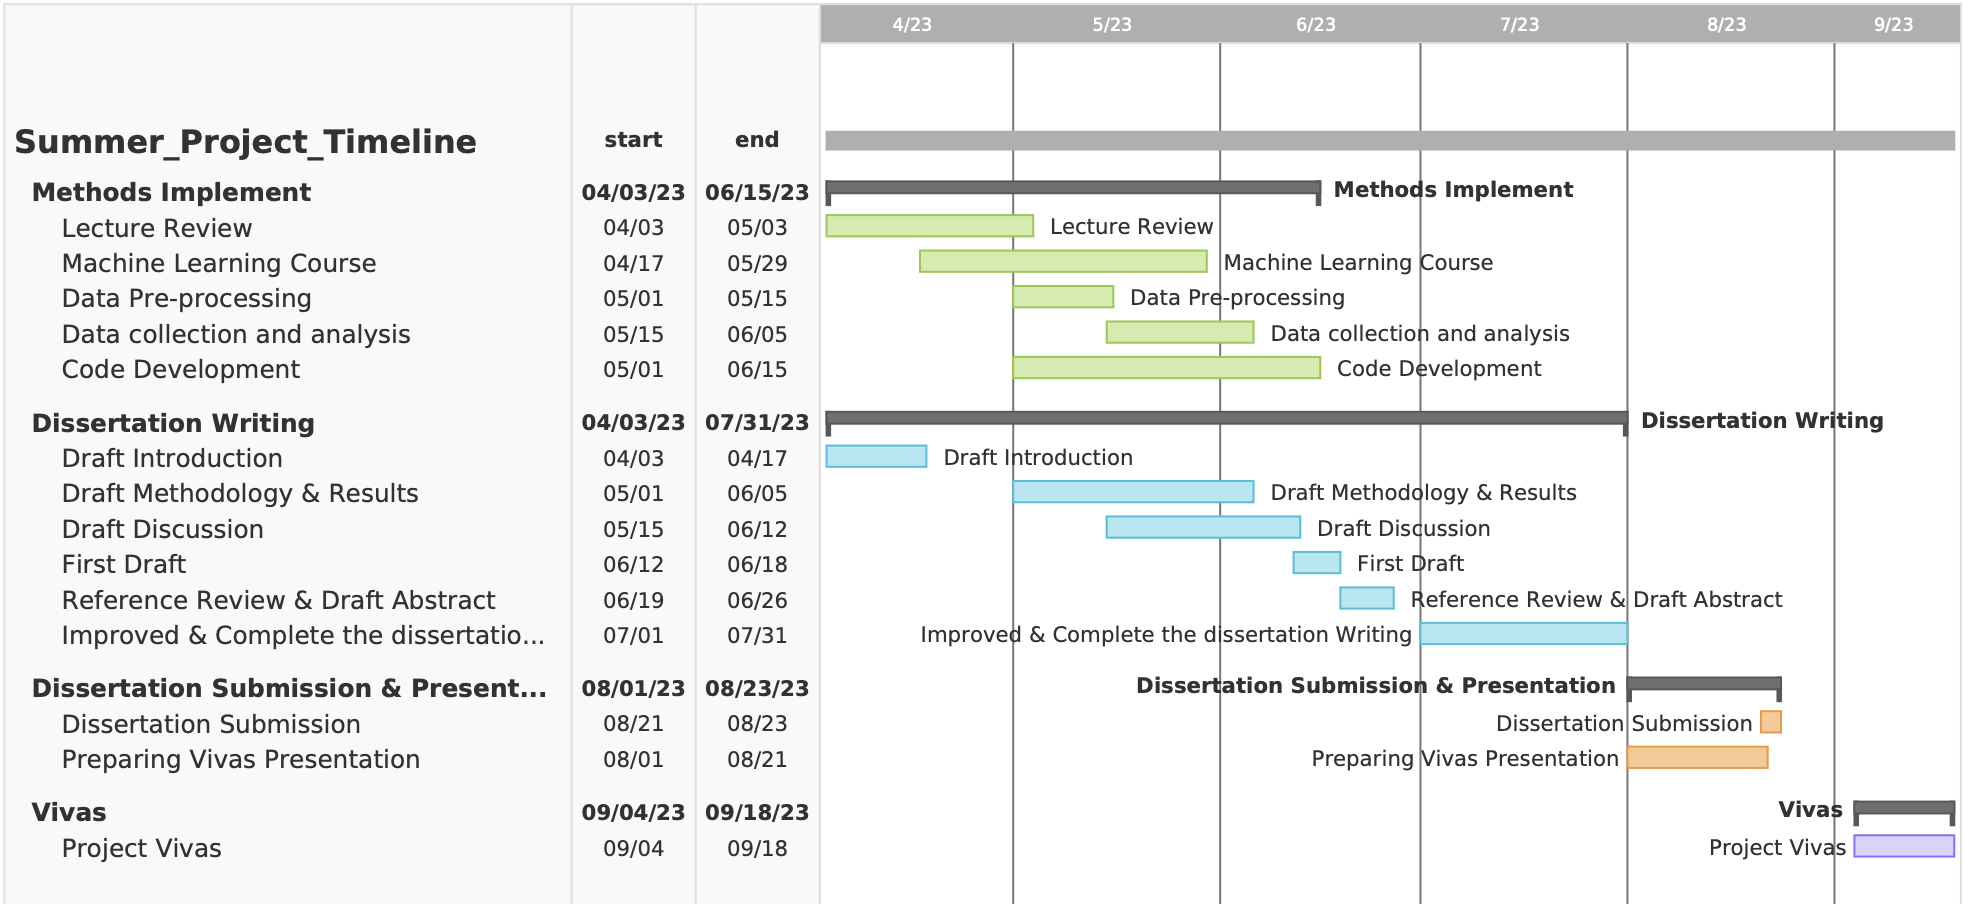
\includegraphics[scale=0.5]{../data/Gantt.png}\\
\vspace{-0.7cm}

\section{Budget}\\
\begin{table}[H]
\begin{tabular}{llc}
Item               & Price (£) & Justification                                   \\
2TB/5TB Hard Drive & 100       & To backup and store all files and big data sets \\
Online Machine Learning Course & 350 & Get more understanding in Machine learning and applied into \\ & &Random Forest modelling \\
Transportation     & 50        & Transportation fee from Silwood to London      
\end{tabular}
\end{table}

\section{Supervisor Declaration}

I have seen and approved the proposal and the budget. \\
\textit{Primary Supervisor: Dr Emma Ransome}\\
Signature:\\
\\
Date: 03/04/2023

\bibliographystyle{apalike}
\bibliography{ref}   
\end{document}